\documentclass[12pt, letterpaper, fleqn]{article}
\usepackage[letterpaper, margin=.75in]{geometry}
\usepackage[utf8]{inputenc}
\usepackage{amsmath}
\usepackage{amssymb}
\usepackage{algorithmicx}
\usepackage{algpseudocode}
\usepackage{algorithm}
\usepackage[english]{babel}
\usepackage{amsthm}
\usepackage{graphicx}
\usepackage{xcolor}
\graphicspath{ {.} }
\usepackage{fancyhdr}
\usepackage{tikz}
\usepackage{hyperref}
\usepackage{cancel}
\newcommand*\circled[1]{\tikz[baseline=(char.base)]{
            \node[shape=circle,draw,inner sep=2pt] (char) {#1};}}
\setlength\parindent{0pt}
\def\fullouterjoin{\mathbin{\ojoin\mkern0mu\bowtie\mkern3mu\ojoin}}

%\pagestyle{fancy}
%\fancyhf{}
%\rhead{Bill Yang}
%\renewcommand{\headrulewidth}{0pt}

\newcommand{\handout}[5]{
   \renewcommand{\thepage}{#1-\arabic{page}}
   \noindent
   \begin{center}
   \framebox{
      \vbox{
%    \hbox to 5.78in { {\bf M328K Number Theory} \hfill #2 }
%       \vspace{4mm}
%       \hbox to 5.78in { {\Large \hfill #5  \hfill} }
%       \vspace{2mm}
%       \hbox to 5.78in { {\it #3 \hfill #4} }
    \hbox to 5.78in { { Bill Yang} \hfill {Due: #2} }
       \vspace{4mm}
       \hbox to 5.78in { {\Large \hfill #5  \hfill} }
       \vspace{2mm}
       \hbox to 5.78in { {#3 \hfill #4} }
      }
   }
   \end{center}
   \vspace*{4mm}
}

\newcommand{\ho}[5]{\handout{#1}{#2}{#3}{Instructor: #4}{Homework #1}}

\begin{document}
  \ho{9}{4/17/20}{CS386D Database Systems}{Daniel Miranker} \\

  \section{Part 1}
\begin{center}
\begin{tabular} { |c | c | c | c | }
  \hline
  \multicolumn{2}{|c|}{Local}  & \multicolumn{2}{|c|}{AWS} \\
  \hline
  Seconds & Bandwidth & Seconds & Bandwidth \\
  \hline
   115.4 & 11.1 Mbytes/second & 95096.3 &  13.9 Kbytes/second \\
  \hline
\end{tabular}
\end{center}


  \section{Part 2}
  30 million rows \\
  7680000000 bytes or 7.15 Gbytes\\\\

  \textbf{1. A}
  Yes, merge-join is chosen. \\
  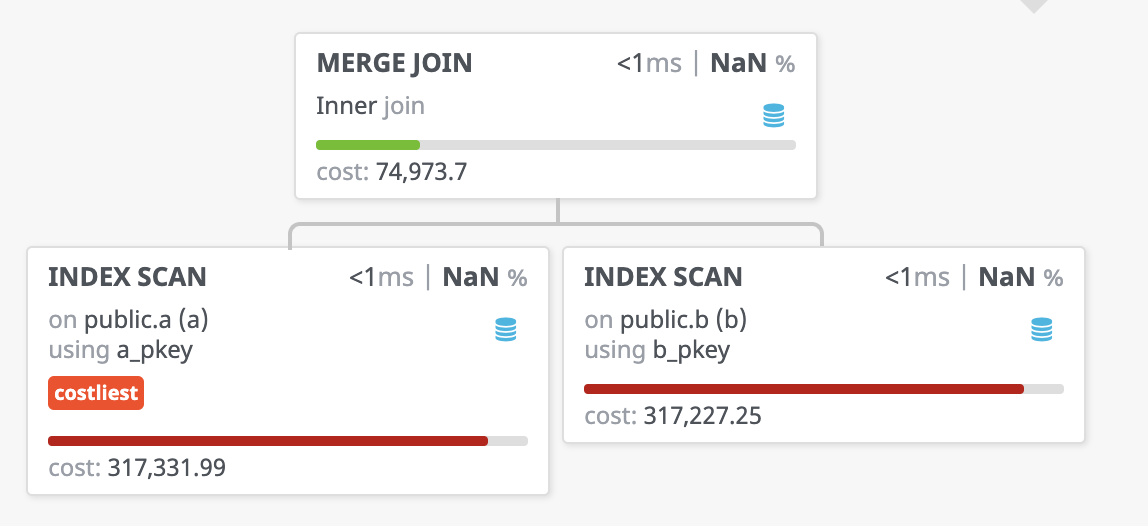
\includegraphics[scale=0.5]{query_pics/1.png} \\
  Using Select A.pk, B.pk\\
  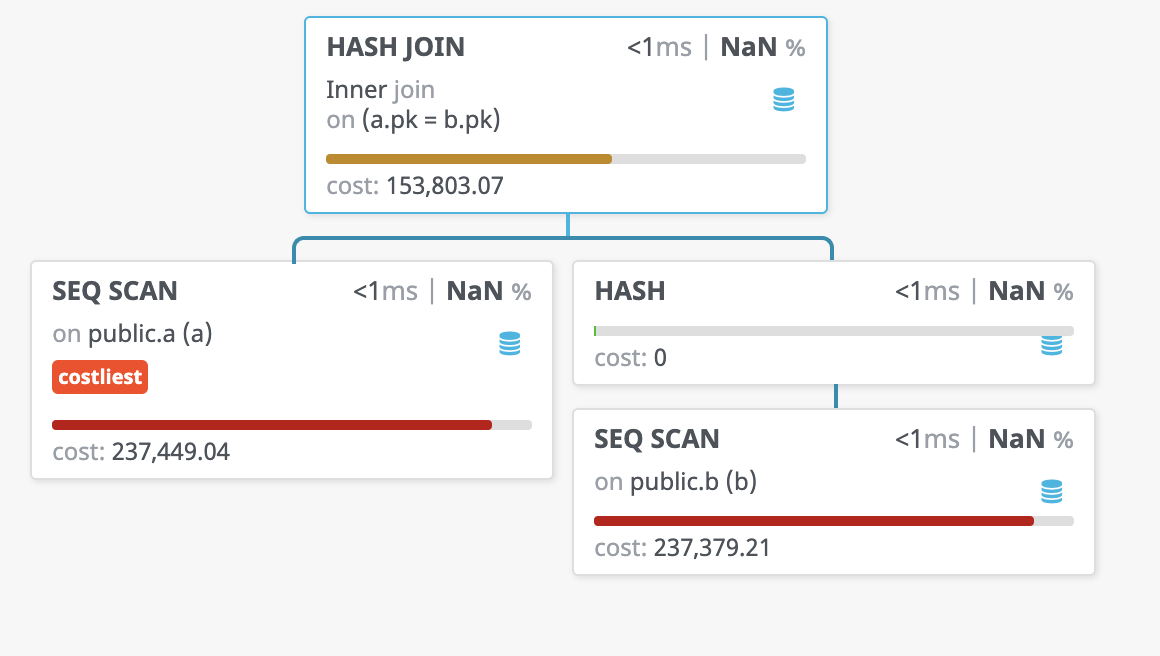
\includegraphics[scale=0.5]{query_pics/1b.png} \\\\

  \textbf{2. B}
  Hash Join \\
  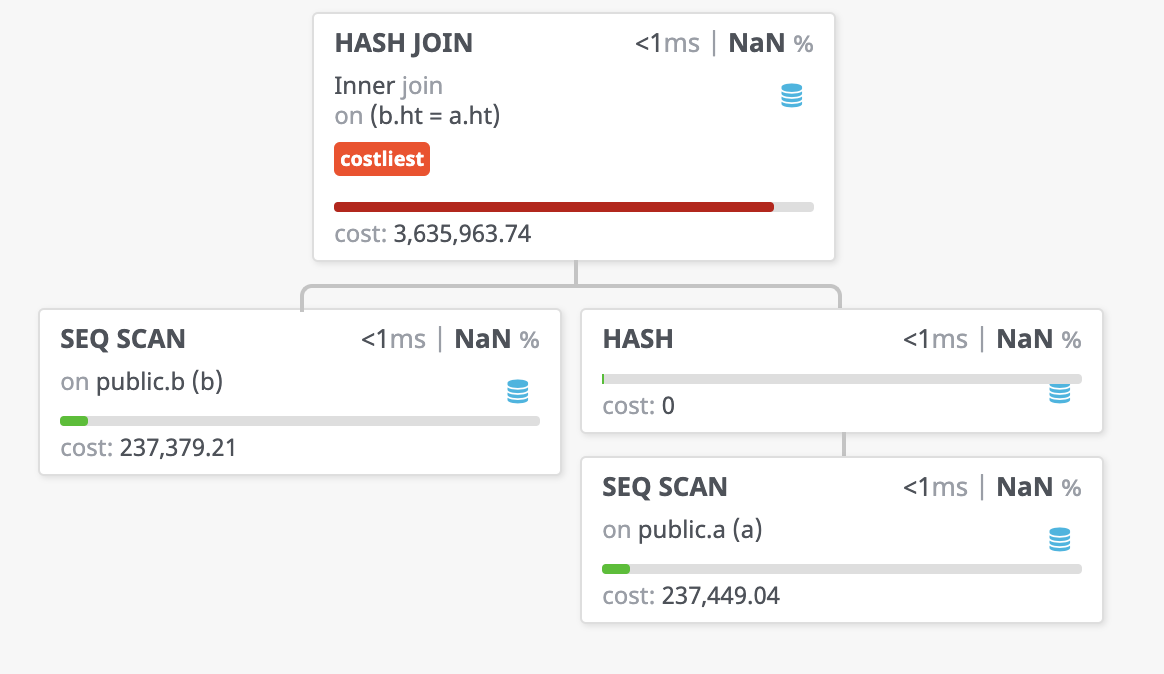
\includegraphics[scale=0.5]{query_pics/2.png} \\
  Using Select A.ht, B.ht\\
  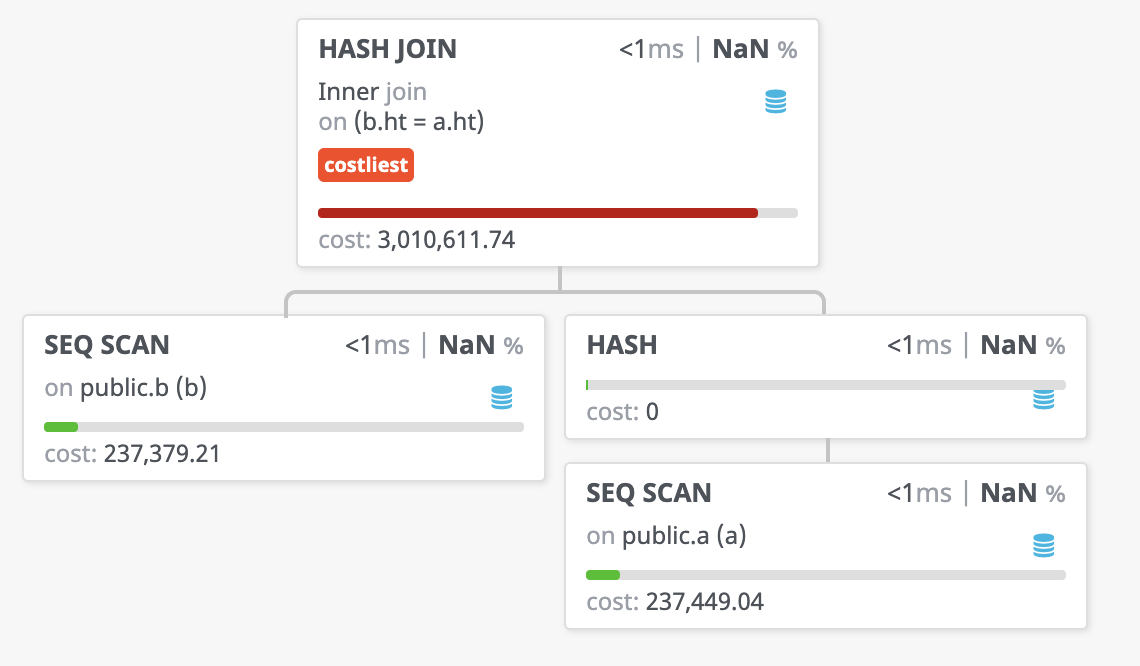
\includegraphics[scale=0.5]{query_pics/2b.png} \\\\


  \textbf{3. C}
  The secondary index does not affect the join order and algorithm for this
  value.\\
  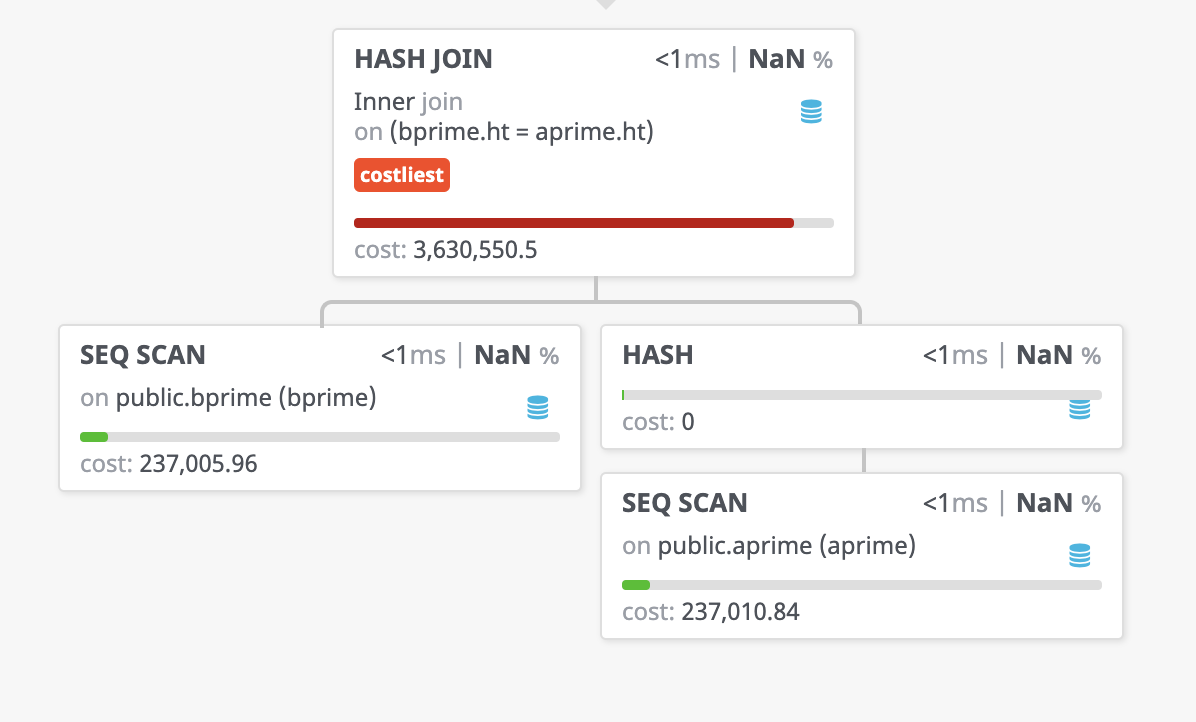
\includegraphics[scale=0.5]{query_pics/3.png} \\
  Using Select Aprime.ht, Bprime.ht\\
  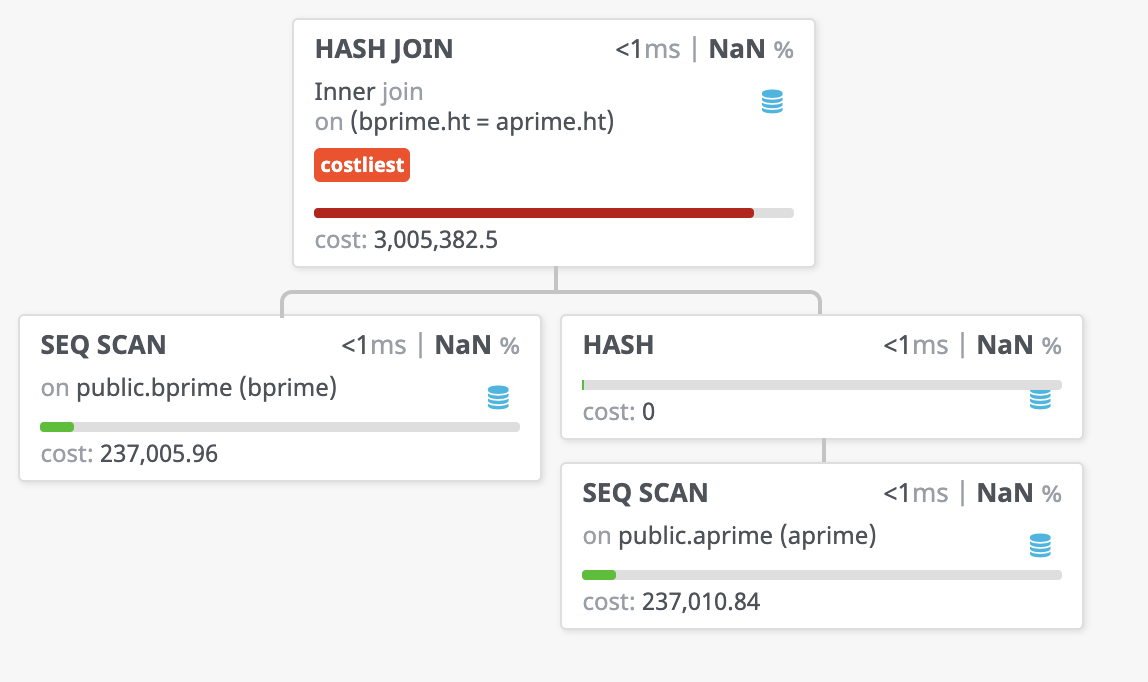
\includegraphics[scale=0.5]{query_pics/3b.png} \\\\

  \textbf{4. D}
  Merge Join was used\\
  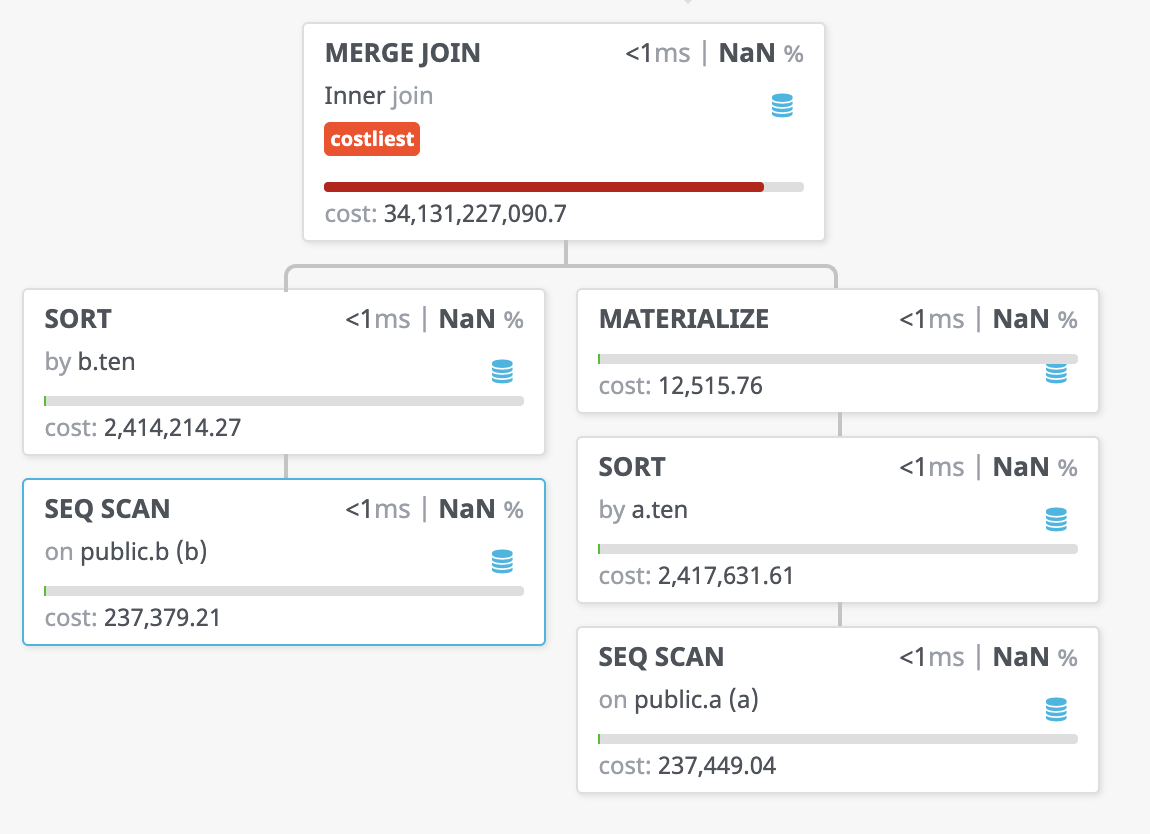
\includegraphics[scale=0.5]{query_pics/4.png} \\
  Using Select A.ten, B.ten\\
  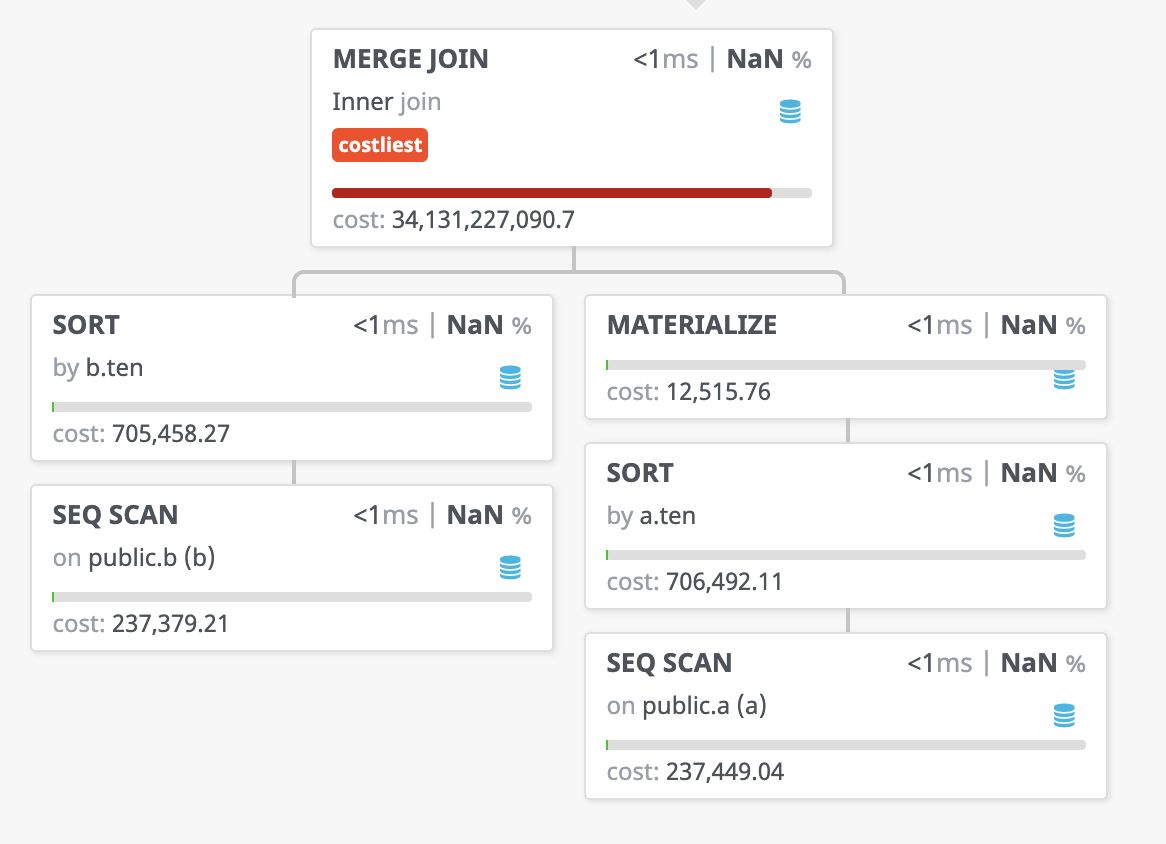
\includegraphics[scale=0.5]{query_pics/4b.png} \\\\

  \textbf{5. E}
  Merge Join was used. \\
  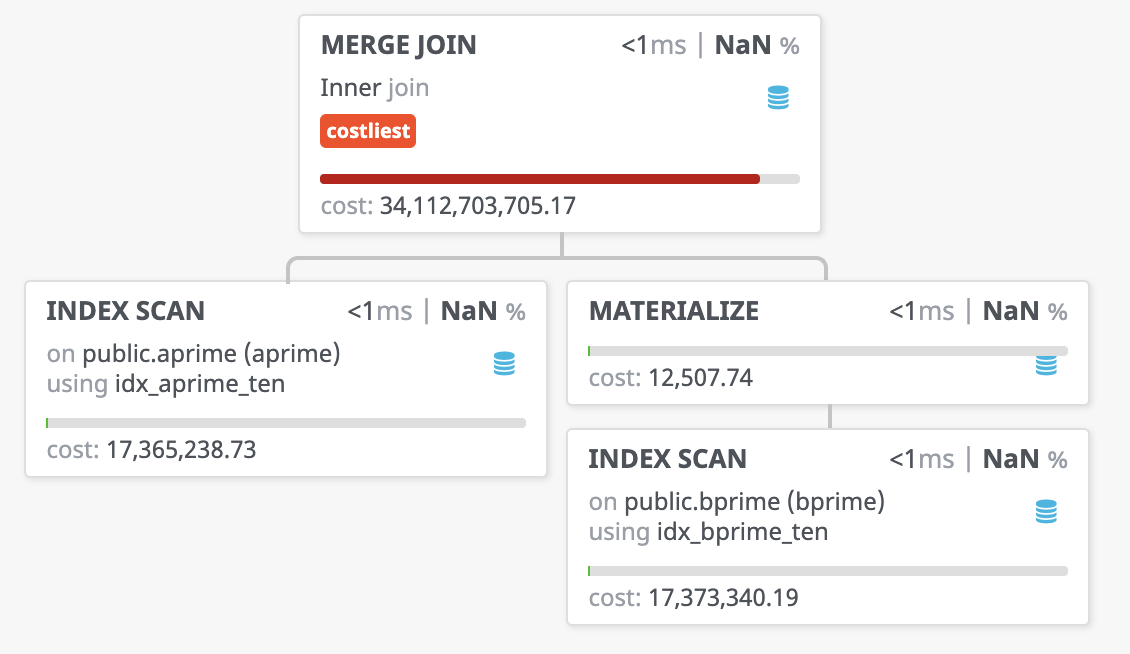
\includegraphics[scale=0.5]{query_pics/5.png} \\
  Using Select Aprime.ten, Bprime.ten\\
  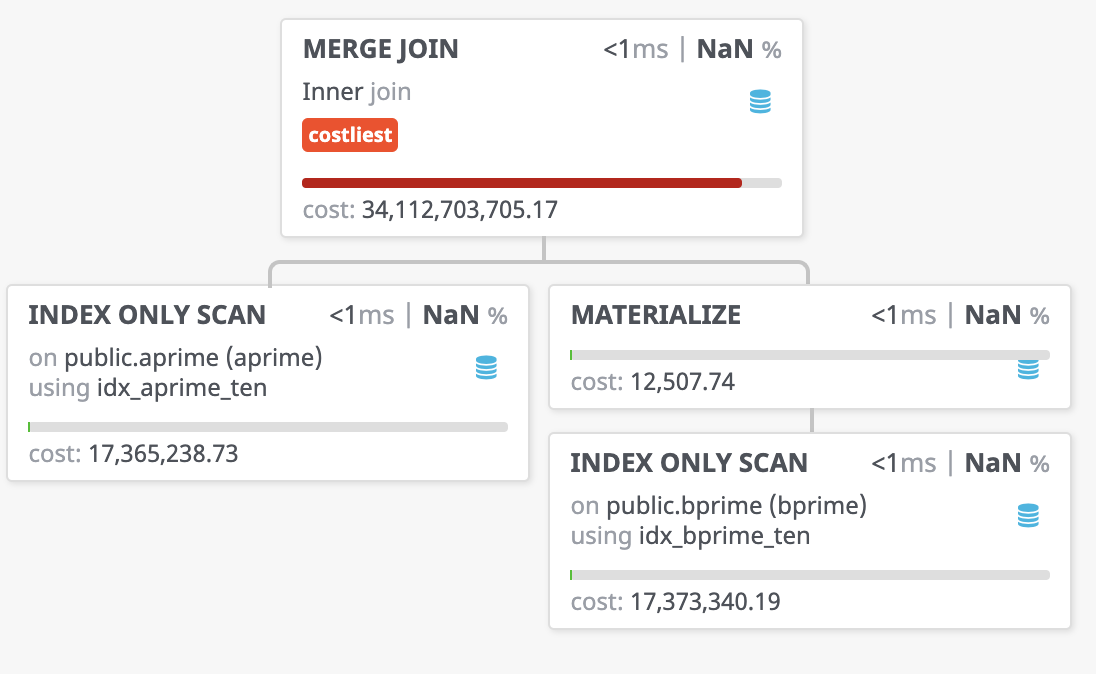
\includegraphics[scale=0.5]{query_pics/5b.png} \\\\
  
  \textbf{F} Yes the optimizer ignores the order I wrote the query, and does its
  own order independently. \\
  \textbf{6. }\\
  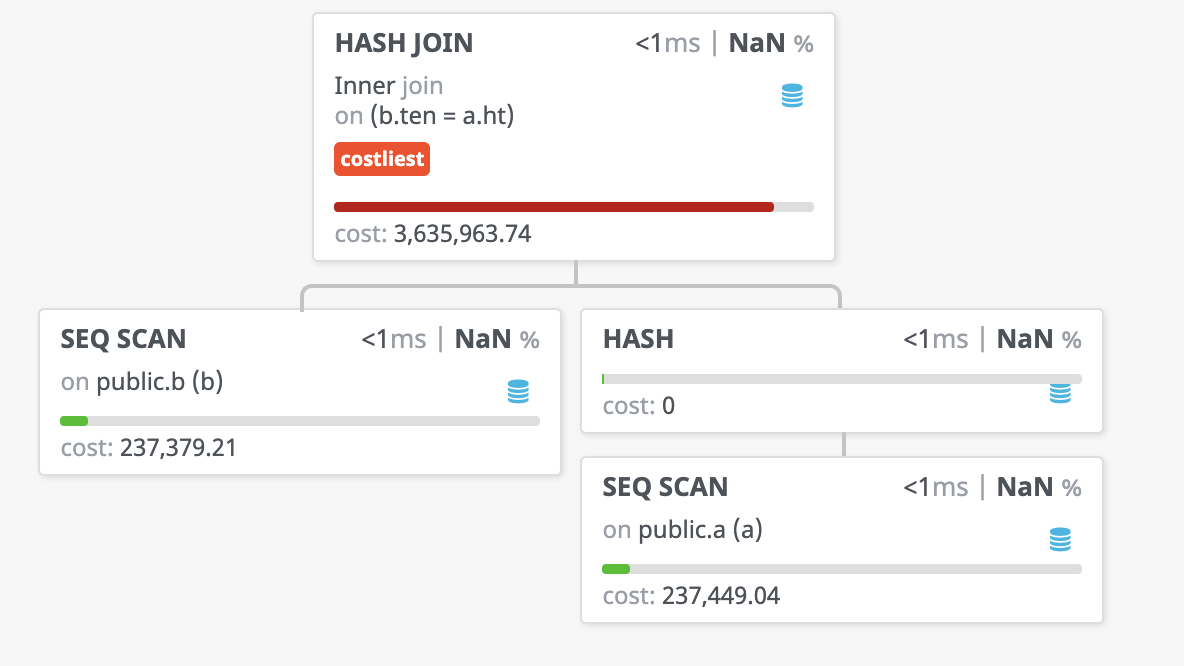
\includegraphics[scale=0.5]{query_pics/6.png} \\
  \textbf{7. }\\
  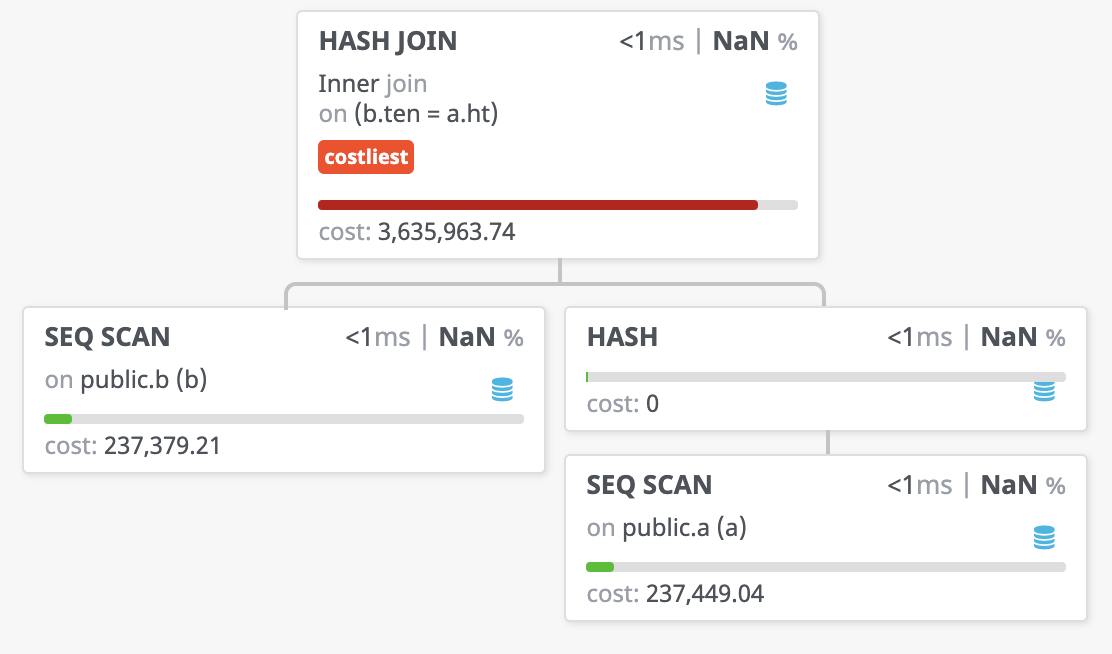
\includegraphics[scale=0.5]{query_pics/7.png} \\\\

  \textbf{G} The optimizer still does its own order for joins independent of how
  I wrote the query.\\
  \textbf{8. }\\
  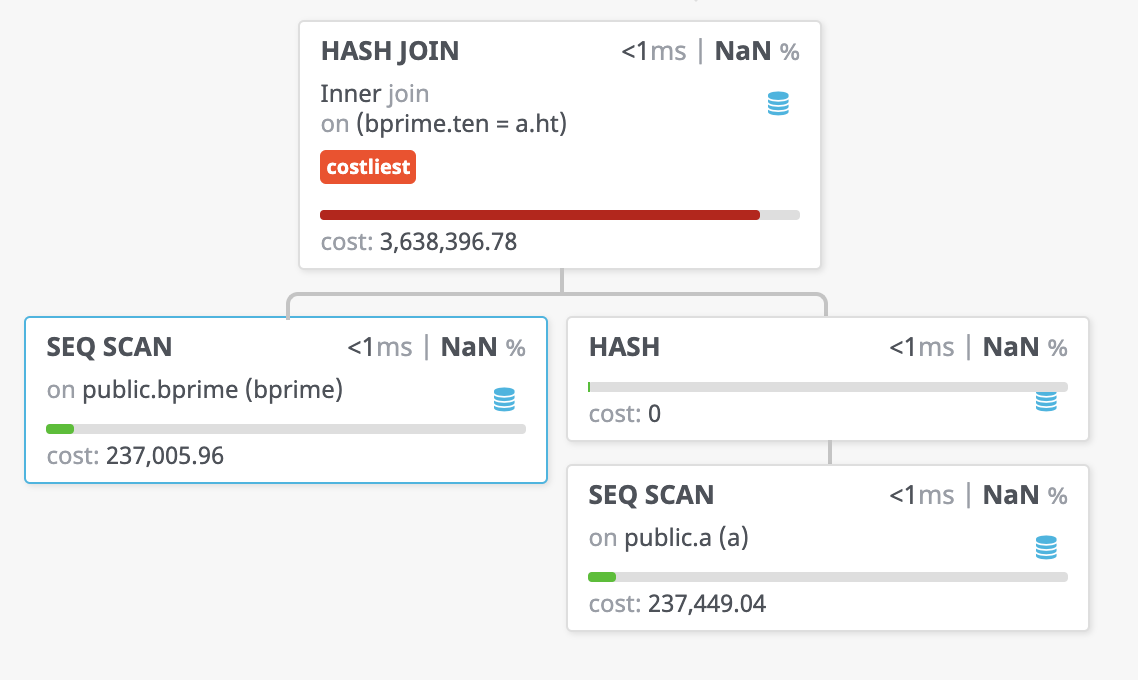
\includegraphics[scale=0.5]{query_pics/8.png} \\
  \textbf{9. }\\
  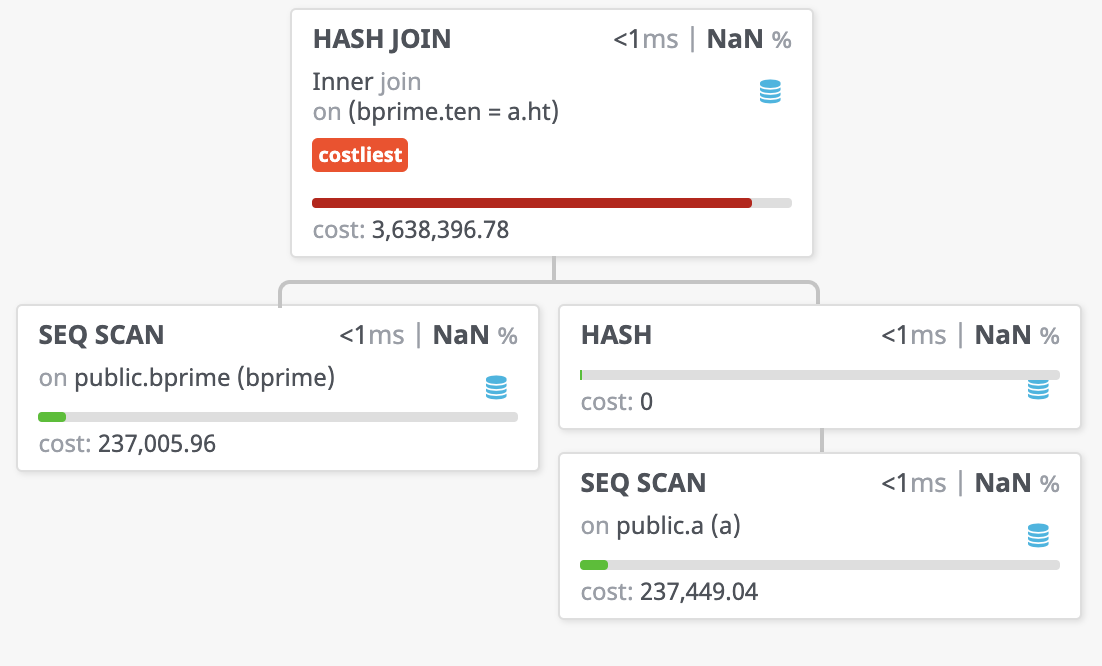
\includegraphics[scale=0.5]{query_pics/9.png} \\\\

  \textbf{H. }\\
  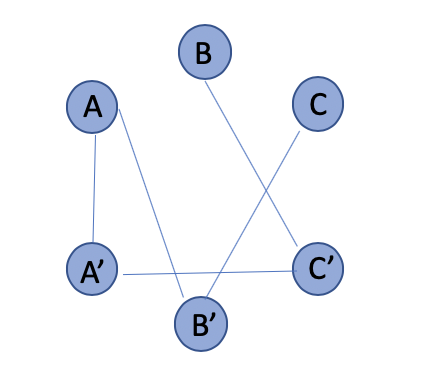
\includegraphics[scale=0.4]{query_pics/23query.png} \\

  \textbf{I. }\\
  	3231988424291524 rows\\\\
  \textbf{23. }\\
  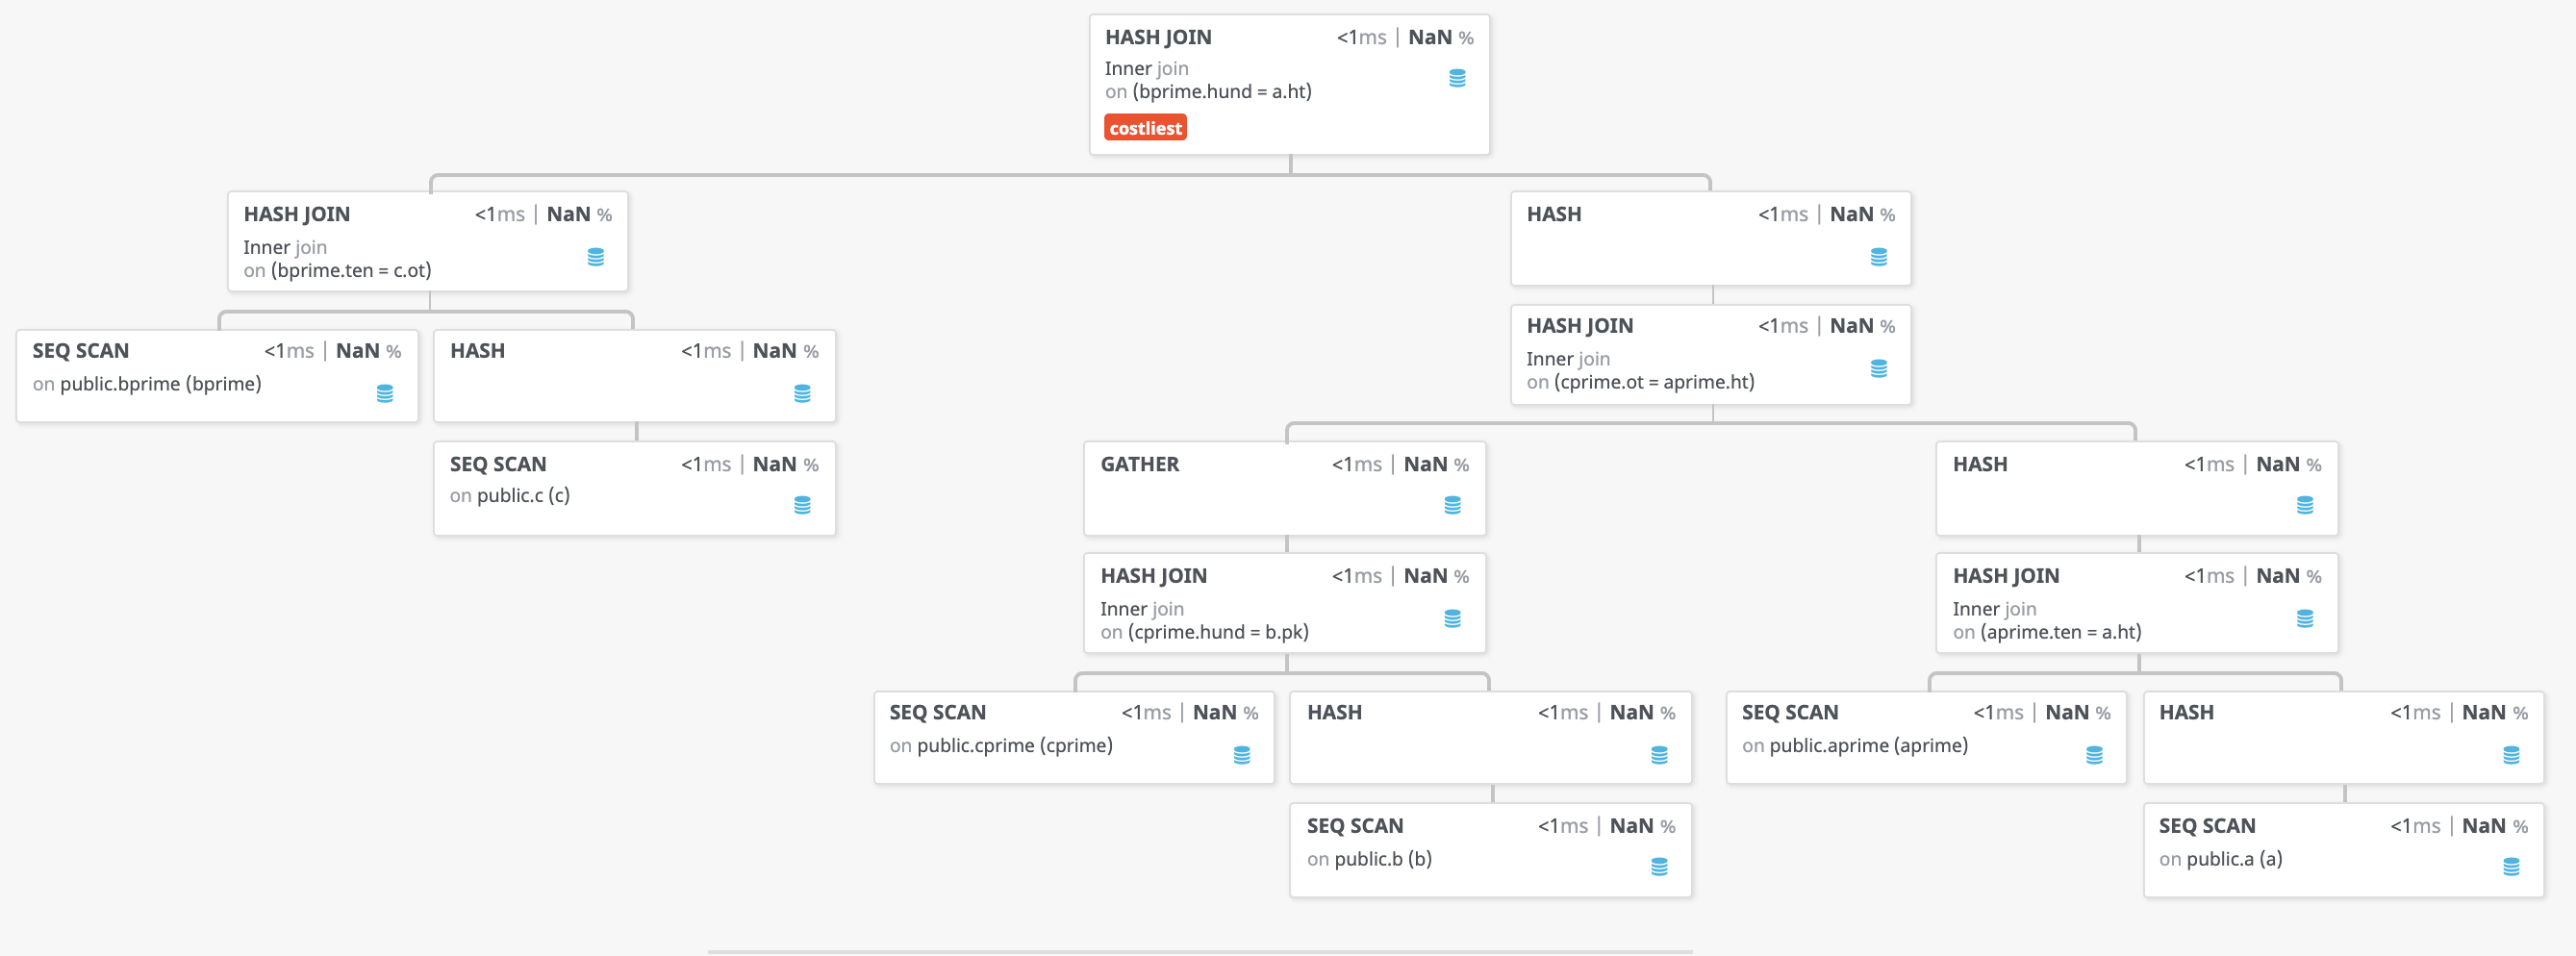
\includegraphics[scale=0.4]{query_pics/23.png} \\
  With the select clause only containing the included arguments\\
  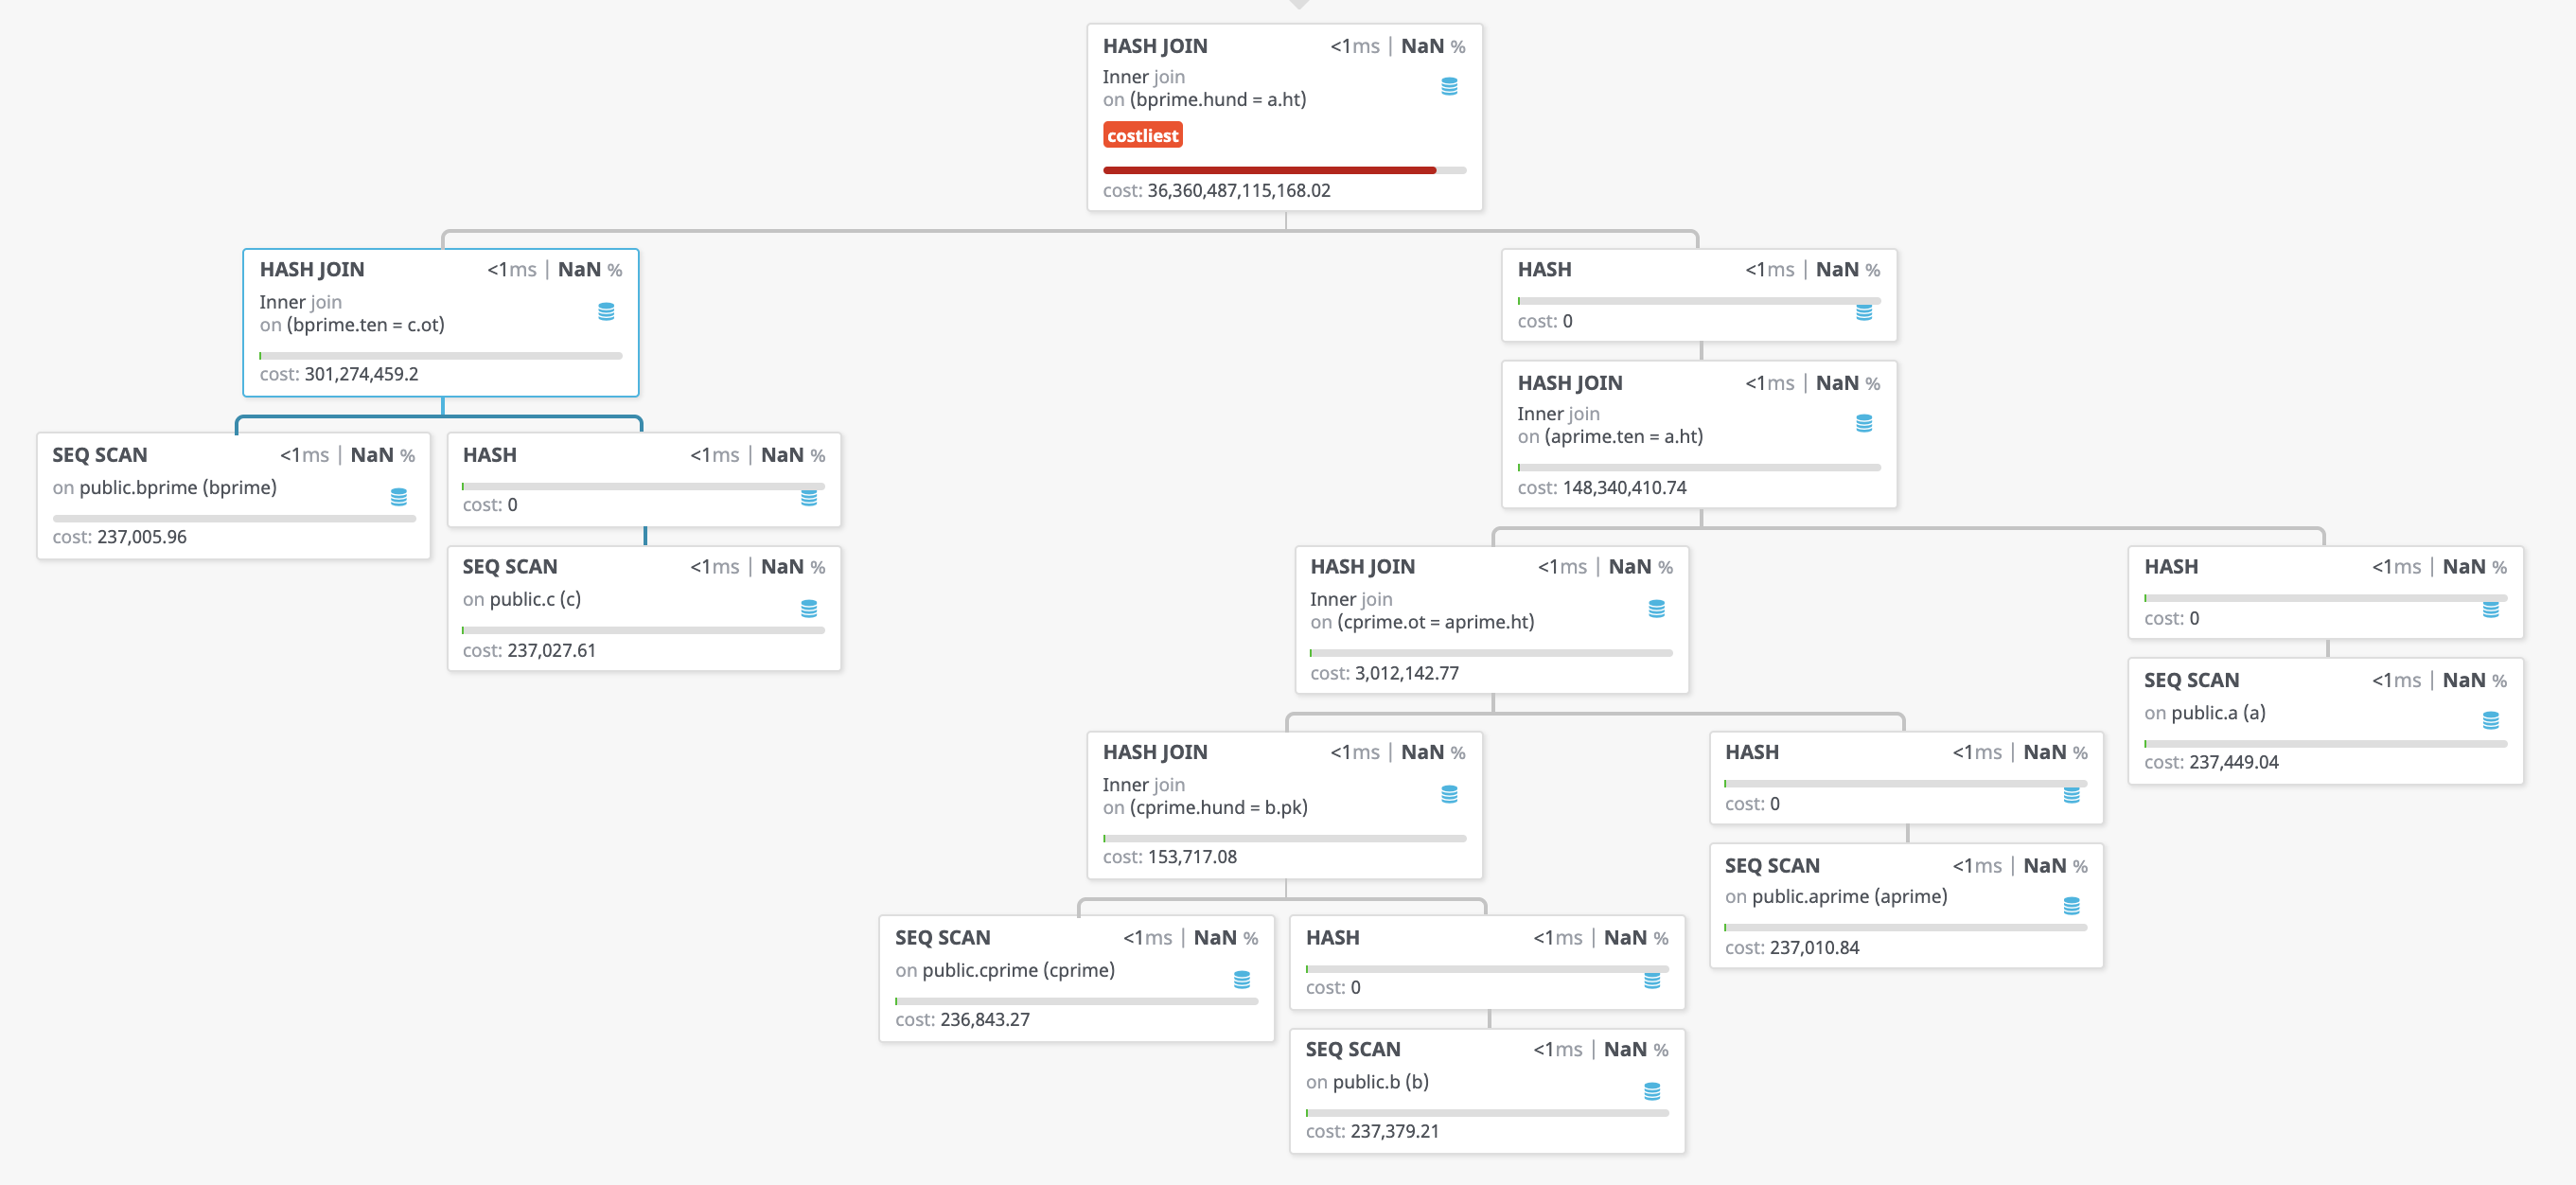
\includegraphics[scale=0.4]{query_pics/23b.png} \\\\

  \textbf{H. }\\
  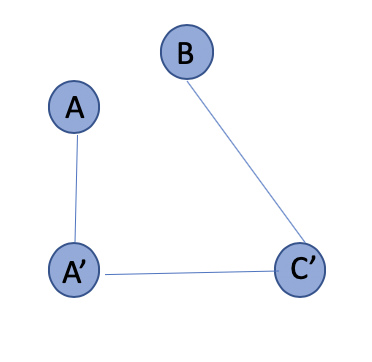
\includegraphics[scale=0.4]{query_pics/24graph.png} \\

  \textbf{I. }\\
  	18897218018647 rows\\\\


  \textbf{24. }\\
  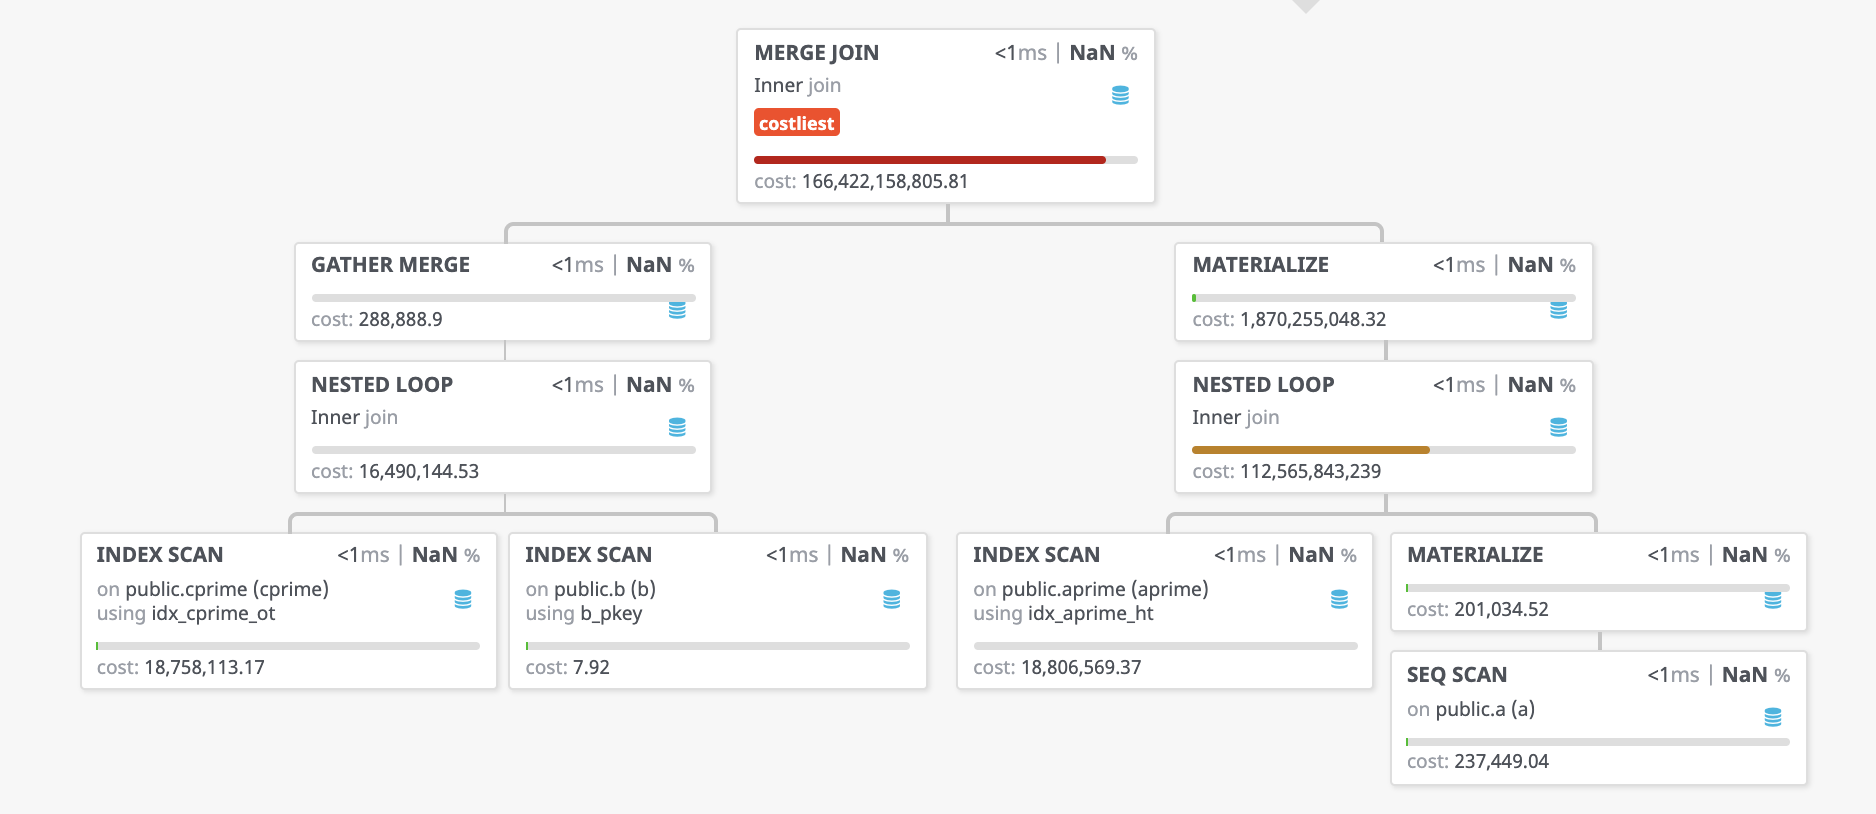
\includegraphics[scale=0.4]{query_pics/24.png} \\
  With the select clause only containing the included arguments\\
  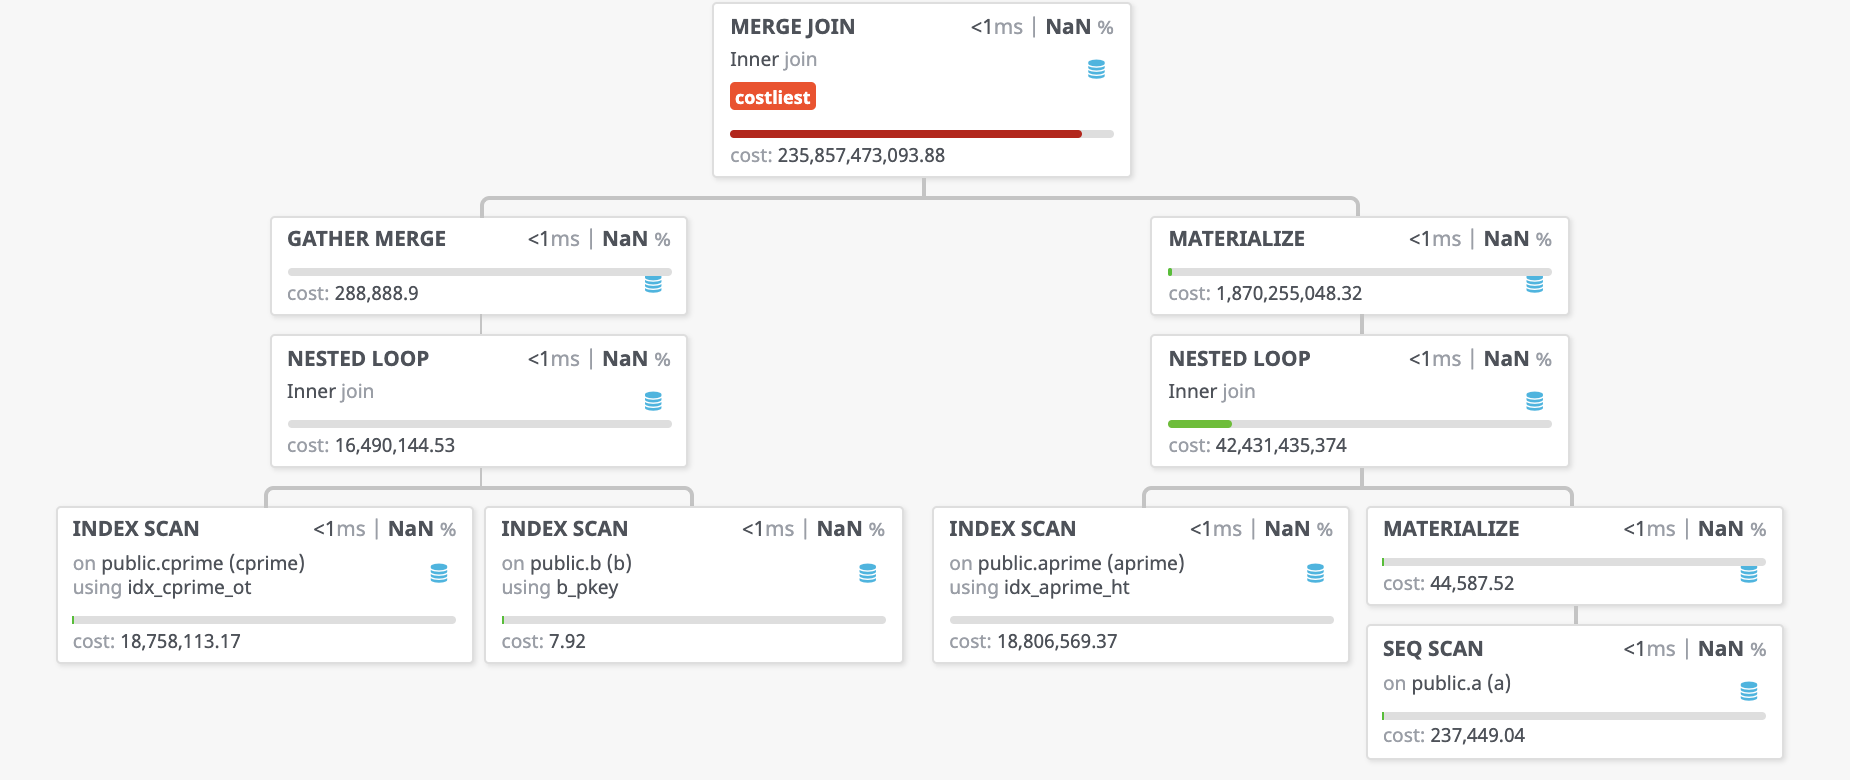
\includegraphics[scale=0.4]{query_pics/24b.png} \\\\
\end{document}
